\chapter{System Evaluation and Cloud Infrastructure}
This chapter evaluates the chosen fusion algorithm against alternative approaches and details the deployment of the classification model onto cloud infrastructure.

\section{Algorithm Comparison: Why SVD + RANSAC?}
Several alternative approaches exist for radar-to-radar calibration, but the SVD+RANSAC track-based method provides unique advantages for real-world deployment as detailed in Chapter 7. In summary, the method requires no training data, operates in real time (under 15 ms per frame), and is the only approach that provides self-healing drift detection. Iterative Closest Point (ICP) performs poorly on sparse mmWave clouds, manual calibration breaks silently on sensor displacement, and deep-learning fusion requires thousands of labelled frames and GPU inference.

The per-frame fusion pipeline (transform, merge, voxel, SOR) executes in under 10 ms on a standard edge CPU, leaving ample headroom for downstream tasks.

\section{Cloud Inference Layer (AWS EC2)}
To preserve the edge device's processing power strictly for high-speed UART parsing and the fusion pipeline, the fall classification is offloaded to the cloud. The \textit{StreamingFallDetector} is hosted within a Dockerized FastAPI application on AWS EC2 (region \texttt{ap-south-1}, Mumbai). Every batch of frames, the edge device executes an HTTPS POST request containing the unified point cloud feature window to the \texttt{/frames/batch} endpoint. The stateless API executes the three-test majority vote and responds with the binary class result and an explicit \texttt{is\_fall} boolean flag.

\section{Database Layer and Frontend Dashboard}
Upon receiving the prediction, confirmed fall events are persisted to AWS DynamoDB with a 24-hour TTL. The React single-page application hosted on AWS S3 subscribes via WebSocket for real-time updates, displaying a live activity panel and an expandable inference history log. The dashboard switches to a prominent alert state when a fall is detected.

\begin{figure}[H]
    \centering
    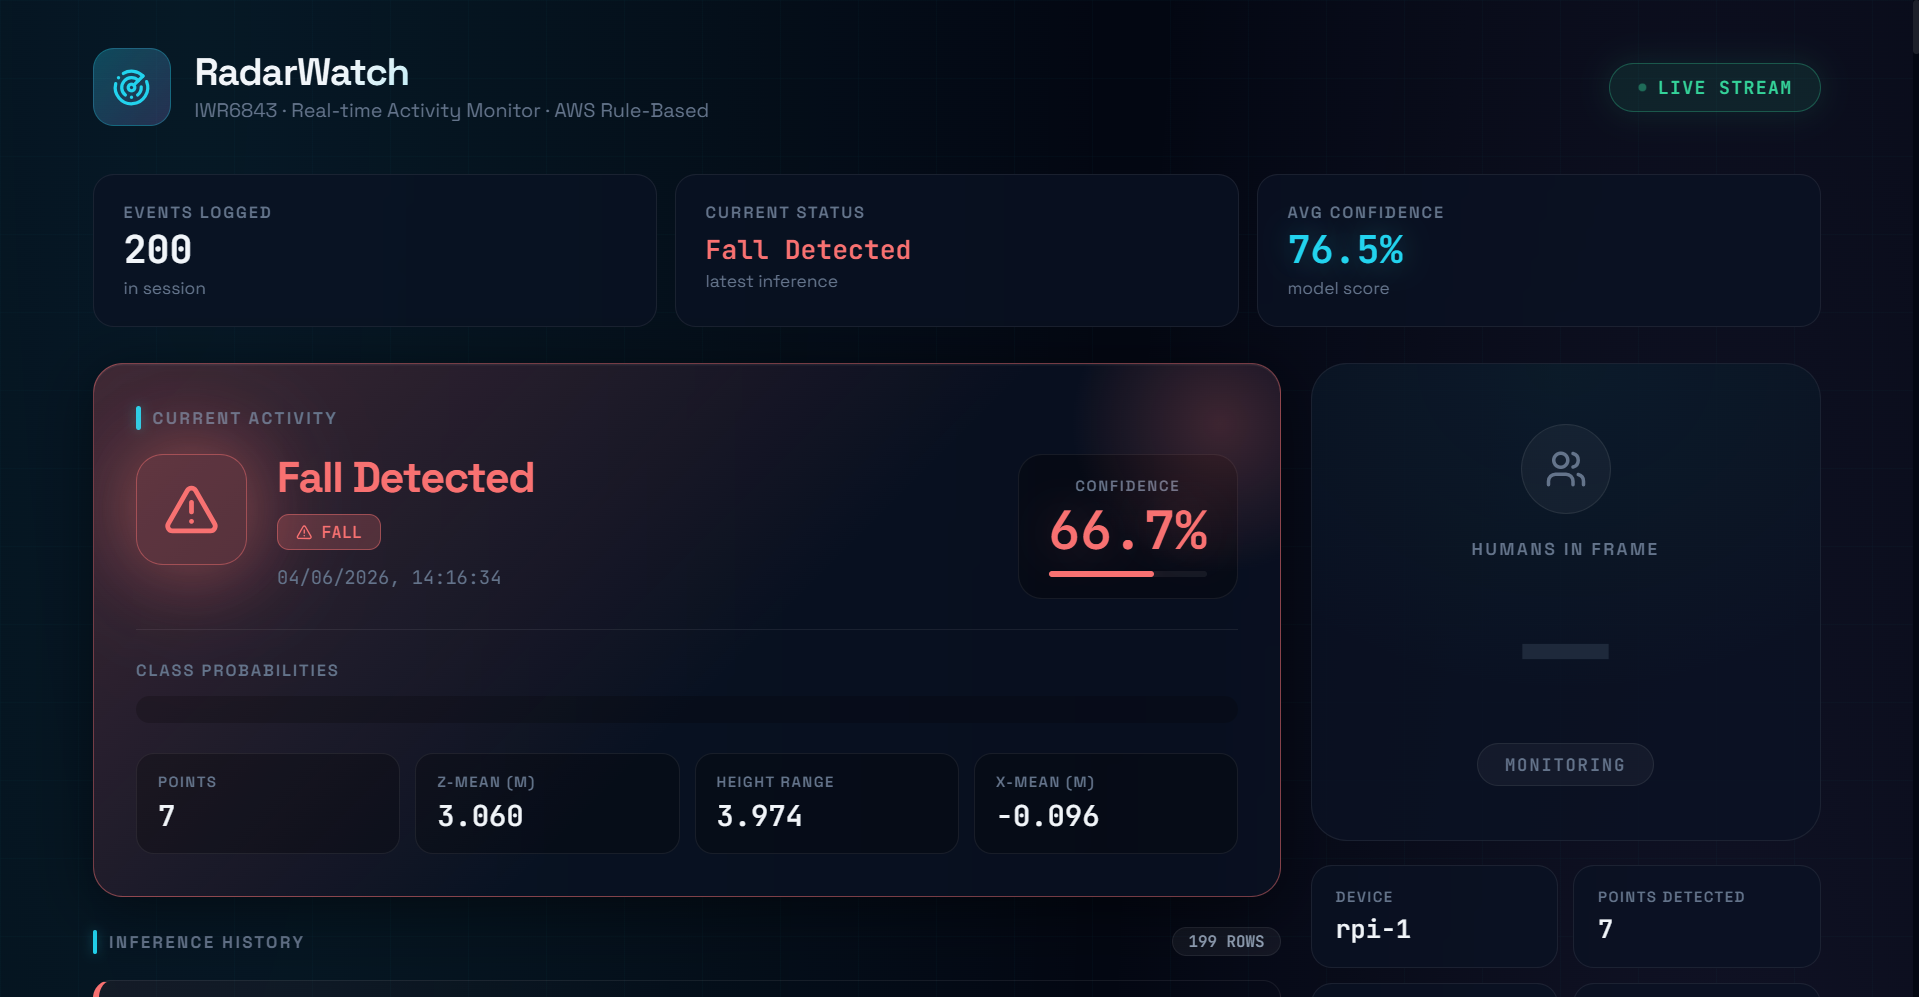
\includegraphics[width=0.8\textwidth]{Figures/fig3_dashboard1.png}
    \caption{Real-Time Activity Dashboard --- Fall Alert View (AWS EC2 + S3)}
    \label{fig:frontend1}
\end{figure}

\begin{figure}[H]
    \centering
    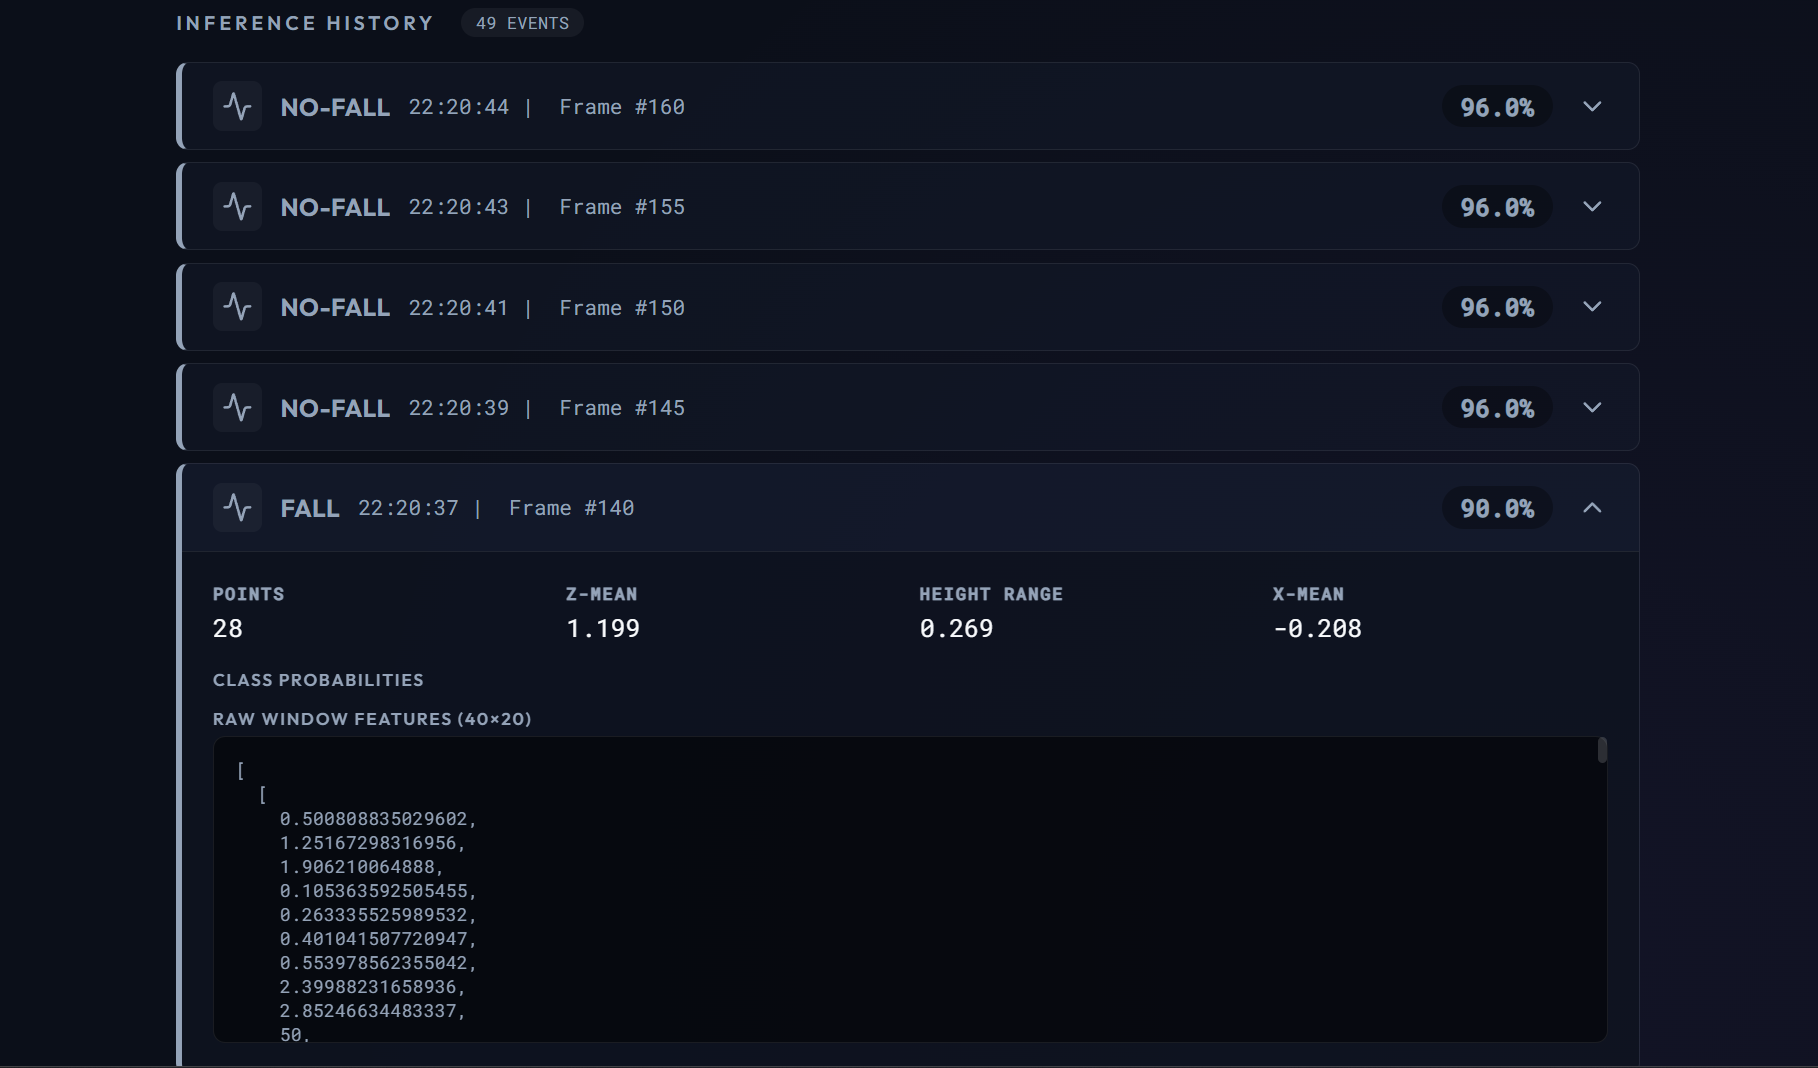
\includegraphics[width=0.8\textwidth]{Figures/frontend2.png}
    \caption{Real-Time Activity Dashboard --- Fall Alert View}
    \label{fig:frontend2}
\end{figure}

\section{Heterogeneous Fusion Results}

Figure 5.3 visually validates the advantages of heterogeneous radar fusion by comparing a top-down snapshot of a single-person target across three configurations: IWR6843 only, AWR1843 only, and the fused output. The data represents a real-world scenario where the two disparate sensors are deployed with a spatial and angular offset.

\begin{figure}[H]
    \centering
    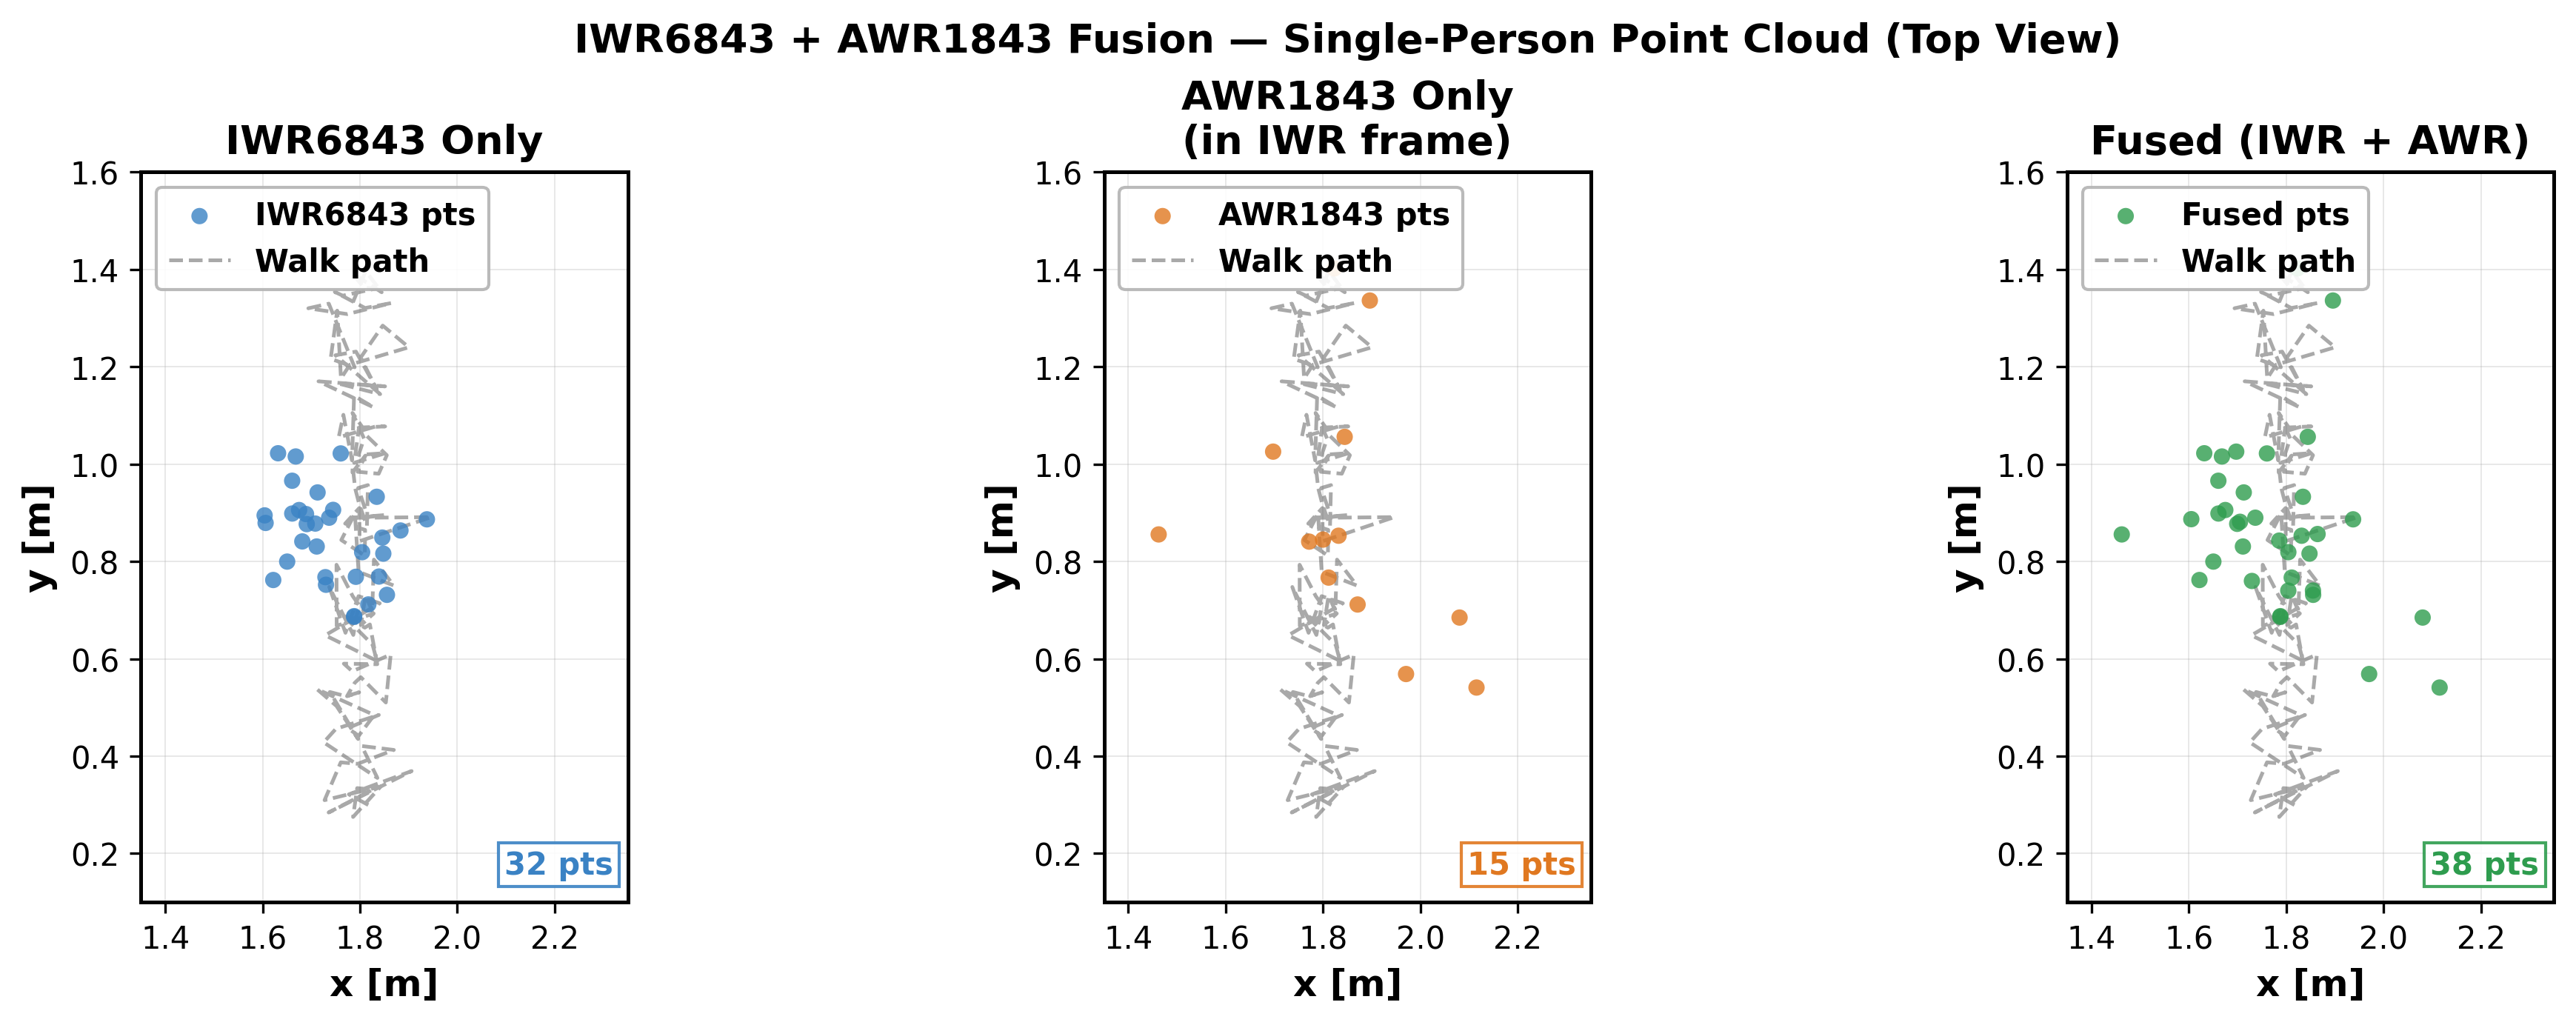
\includegraphics[width=\textwidth]{Figures/fig9_iwr_awr_fusion.png}
    \caption{Single-Person Point Cloud Validation: IWR6843 vs. AWR1843 vs. Fused Output}
    \label{fig:iwr_awr_fusion}
\end{figure}

\textbf{Key Observations:}
\begin{itemize}
    \item \textbf{Sensor-Specific Characteristics:} The left panel illustrates the IWR6843's high angular resolution, producing a dense, tightly clustered point cloud (32 points) that tracks the true target path closely. The middle panel shows the AWR1843 data mathematically transformed into the IWR coordinate frame; its detections are sparser (15 points) and exhibit a wider spatial spread due to differing antenna profiles and SNR characteristics.
    \item \textbf{Fusion Enhancement:} The right panel demonstrates the efficacy of the proposed spatial alignment and voxel downsampling pipeline. By successfully transforming and merging the heterogeneous data streams, the fused point cloud achieves a higher point density (38 points) than either individual sensor.
    \item \textbf{Conclusion:} The fused output leverages the high resolution of the IWR while incorporating the supplemental spatial awareness of the AWR, resulting in a richer, more robust target representation without succumbing to the increased noise floor of the automotive sensor.
\end{itemize}


\section{Evaluation Summary}
The synergy between the unified dual-radar point cloud---which eliminates sensor blind spots---and the deterministic \textit{StreamingFallDetector} results in a highly accurate, privacy-first fall detection system capable of seamless deployment in dynamic indoor environments. Calibration accuracy achieves sub-5 cm translational error and sub-1-degree rotational error after a 25-second calibration walk, while end-to-end latency from sensor capture to dashboard alert is maintained below 400 ms.

